\documentclass{ieeetj}
\newcommand{\seclogo}{}
\usepackage{cite}
\usepackage{amsmath,amssymb,amsfonts}
\usepackage{listings}
\usepackage{algorithmic}
\usepackage{graphicx,color}
\usepackage{textcomp}
\usepackage{hyperref}
\usepackage{float}
\usepackage[table,xcdraw]{xcolor}
\definecolor{blau}{RGB}{198, 220, 255} 
\definecolor{gris}{RGB}{176, 176, 176}
\definecolor{verd}{RGB}{ 173, 240, 199}

\hypersetup{hidelinks=true}
\usepackage{algorithm,algorithmic}
\lstset{
    language=Java,
    basicstyle=\ttfamily\small,
    keywordstyle=\bfseries\color{blue},
    stringstyle=\color{red},
    morecomment=[l][\color{magenta}]{//},
    frame=single,
    breaklines=true,
    showstringspaces=false,
    tabsize=1,
}
\def\BibTeX{{\rm B\kern-.05em{\sc i\kern-.025em b}\kern-.08em
    T\kern-.1667em\lower.7ex\hbox{E}\kern-.125emX}}
\AtBeginDocument{\definecolor{tmlcncolor}{cmyk}{0.93,0.59,0.15,0.02}\definecolor{NavyBlue}{RGB}{0,86,125}}

% Definim el logo
\def\OJlogo{
    \vspace{-14pt} % Espai negatiu per pujar el logo
    
\includegraphics[height=0.96cm]{png/logo.png}}

\begin{document}
\receiveddate{////}
\publisheddate{/////}
\currentdate{//////}

\title{Algorismes àvids o de curta mira: COMPRESSOR D'ARXIUS}

\author{Josep Ferriol, Daniel García, Khaoula Ikkene, Biel Perelló} \affil{Universitat de les Illes Balears, Departament d'Enginyeria Informàtica} \corresp{Autor de contacte: Daniel García (email: daniel.garcia19@estudiant.uib.es)}



\begin{abstract} 
Aquest document introdueix un programa de compressió i descompressió d'arxius de qualsevol tipus, basat en l'algorisme de Huffman, conegut per la seva capacitat de compressió sense pèrdua de dades. Aquesta solució s'aplica a través d'una estructura que garanteix la integritat de la informació original mentre redueix eficientment el tamany dels fitxers.

El programa se centra en la implementació de l'algorisme de Huffman i inclou els components necessaris per a la compressió i la descompressió, així com diverses implementacions de cues de prioritat per comparar-ne l'eficiència en diferents escenaris. Aquestes comparacions són especialment rellevants per determinar l'impacte de cada estructura sobre el rendiment general del sistema.\newline

L'aplicació segueix el patró arquitectònic de model-vista-controlador treballat durant el curs i ofereix una interfície gràfica d'usuari (GUI) amigable per facilitar la interacció amb el programa. A més, incorpora un ús eficient de la concurrència per optimitzar el temps d'execució, especialment en operacions amb grans volums de dades.

Al llarg d'aquest document, es detallen les funcionalitats principals del programa i es presenten resultats comparatius que analitzen el comportament de les cues de prioritat i l'eficiència de la compressió. Aquestes mesures aporten una visió clara del rendiment i de la utilitat pràctica del sistema.
\end{abstract}

\begin{IEEEkeywords}
Algorismes àvids, compressió sense pèrdua, codificació de Huffman, entropia de Shannon, cues de prioritats, heap binari, Fibonacci heap, Rank-Pairing heap, Model–Vista–Controlador (MVC), concurrència en Java, estructura òptima de codificació.
\end{IEEEkeywords}


\maketitle


\section{Introducció}
La rapidesa amb què creix el volum d’informació digital fa imprescindible l’ús de tècniques de compressió eficients que redueixin l’espai d’emmagatzematge i el temps de transmissió sense perdre fidelitat. 

La pràctica que es presenta consisteix en el \textbf{disseny i la implementació d’un compressor–descompressor de fitxers} que, partint d’una anàlisi estadística del contingut, construeix un arbre de Huffman orientat a la \emph{mínima entropia} i obté codis canònics compactes. El projecte abraça diverses àrees del currículum:

\begin{itemize}
  \item \textbf{Teoria de la informació}: càlcul de l’entropia de Shannon i comparació amb la longitud mitjana dels codis per mesurar l’eficiència.
  \item \textbf{Estructures de dades avançades}: experimentació amb tres cues de prioritats (\emph{Binary Heap}, \emph{Rank-Pairing Heap}, etc.) per avaluar-ne l’impacte en el temps de construcció de l’arbre.
  \item \textbf{Concurrència en Java}: paral·lelització del recompte de freqüències i del recorregut de l’arbre per aprofitar processadors multinúcli.
  \item \textbf{Enginyeria del programari}: aplicació del patró \emph{Model–Vista–Controlador} (MVC) i desenvolupament d’una GUI intuïtiva amb Swing.
\end{itemize}

\noindent
En aquest projecte s'ha implementat:
\begin{enumerate}
  \item \textbf{Càrrega i anàlisi de fitxers}: admetre tant text com binaris, calcular la distribució de freqüències i determinar l’entropia del fitxer d’entrada.
  \item \textbf{Construcció òptima de l’arbre}: generar l’arbre de Huffman mitjançant l’estructura de cua triada per l’usuari i derivar-hi un codi canònic que minimitzi l’espai de capçalera.
  \item \textbf{Compressió i descompressió transparents}: convertir l’arxiu original a un format propietari (\texttt{.huf}) que inclou la taula canònica i permet recuperar el contingut sense pèrdua.
  \item \textbf{Interfície gràfica d’usuari}: proporcionar una finestra amb \emph{drag \& drop}, botons d’acció (carregar, comprimir, descomprimir, guardar) i un panell que visualitza l’arbre, les freqüències i els codis assignats.
  \item \textbf{Avaluació de rendiment}: mesurar la taxa de compressió, el temps d’execució  per a cada combinació de \emph{heap} i mida de paraula (8, 16, 32 o 64 bits); representar gràficament les diferències.
 \end{enumerate}

\noindent

\bigskip
\noindent
En conjunt, la pràctica no només aconsegueix comprimir dades de manera eficient, sinó que també serveix com a laboratori per comprovar rendiments de les distintes coes, la modularitat del codi i trobar la mida de la paraula seleccionada idònia en cada cas.

\section{Marc teòric} 


El desenvolupament del compressor–descompressor de Huffman s'assenta sobre un conjunt de conceptes fonamentals de l'algorísmia i la teoria de la informació.  
En aquest capítol es presenten les bases teòriques que justifiquen les decisions d'implementació preses durant el projecte.

Es descriu el funcionament dels \textbf{algorismes àvids}, s'introdueix la \textbf{teoria de la informació}, centrant-se en el concepte d'\emph{entropia de Shannon}, s'exposa el \textbf{mètode de codificació de Huffman}, s'analitza el paper de les \textbf{cues de prioritats} i es presenta l'estructura arquitectònica seguida al projecte: el \textbf{patró Model–Vista–Controlador (MVC)}.

Cada secció d'aquest capítol intenta aprofundir en aquests conceptes, oferint tant el marc teòric com la seva aplicació pràctica dins del context de la compressió de dades.

%--------------------------------------------------------------------
\subsection{Algorismes àvids}\label{subsec:greedy}
%--------------------------------------------------------------------
Un algorisme àvid (\emph{greedy})  construeix la solució pas a pas prenent la millor decisió local disponible i sense retrocedir mai les eleccions anteriors \cite{cormen2022}. 
Aquesta estratègia es fonamenta en dues propietats clau. La primera és l’\textit{optimal substructure}, que indica que la solució òptima global d’un problema es pot obtenir combinant les solucions òptimes dels seus subproblemes. Això assegura que el problema es pot dividir en parts més petites, resoldre-les de manera independent i reconstruir la solució global de forma directa. La segona propietat és la \textit{greedy-choice}, que implica que es pot prendre una decisió local òptima en cada pas\cite{greedy}, i aquesta decisió formarà part de la solució òptima global, sense necessitat de revisitar passos anteriors.\newline

La simplicitat dels algorismes àvids fa que, quan el problema compleix aquestes propietats, s’assoleixi una solució òptima amb cost $O(n \log n)$ o inferior; en altres casos, l’estratègia produeix aproximacions prou bones en temps pràctic (vegeu l’exemple clàssic de l’heurística de canvi mínim o del TSP) \cite{kaplan2013}.

%--------------------------------------------------------------------
\subsection{Teoria de la informació i entropia}\label{subsec:entropy}
%--------------------------------------------------------------------
La teoria de la informació, introduïda per Claude Shannon\cite{shannon1948} el 1948, proporciona el marc matemàtic per mesurar la quantitat d'informació continguda en un missatge o una font de dades. Aquesta disciplina és fonamental en camps com la compressió de dades, la transmissió d'informació i la codificació, ja que permet quantificar els límits teòrics del processament de la informació.\newline

 Un dels conceptes centrals de la teoria de la informació és l'entropia\cite{entropia}, que mesura la incertesa inherent a una font de dades. La cota inferior teòrica que limita qualsevol esquema de compressió sense pèrdua ve donada per l’entropia de Shannon $H(X)$ \cite{shannon1948}. Per a un alfabet discret $X=\{x_i\}$ de probabilitats $p_i$, es defineix com:



\[
H(X) \;=\; -\sum_{i} p_i \log_2 p_i \quad\text{(bits/símbol)}.
\]



L'entropia representa el nombre mitjà de bits necessaris per codificar un símbol de la font en una codificació òptima. En una codificació prefix-free, la longitud mitjana $\bar L$ satisfà $H(X) \le \bar L < H(X)+1$. 

El disseny de codis que "s'acosten" a aquesta cota és, per tant, l'objectiu central de la codificació de Huffman, que cerca reduir al mínim la longitud total dels missatges codificats sense perdre informació.



%--------------------------------------------------------------------
\subsection{Anàlisi amortitzat
}
L'anàlisi amortitzada\cite{amortized} és una tècnica utilitzada en ciències de la computació per analitzar la complexitat temporal mitjana d'algorismes que executen una seqüència d'operacions, on algunes d'aquestes operacions poden tenir un cost computacional més elevat que d'altres. 
L'objectiu és distribuir el cost d'aquestes operacions costoses entre diverses operacions de manera que el cost mitjà de cada operació es mantingui constant o sigui menor.

A diferència de l'anàlisi en el pitjor cas, que només considera l'operació més costosa, l'anàlisi amortitzada té en compte com interactuen les operacions entre elles dins d'una seqüència. Això permet obtenir una estimació més realista del rendiment global de l'algorisme.
%--------------------------------------------------------------------
\subsection{Cues de prioritats}\label{subsec:heaps}
%--------------------------------------------------------------------
La fase de fusió de Huffman requereix extreure iterativament els dos símbols
de menor freqüència d’una cua de prioritats $Q$. Aquestes son les estructures utilitzades:

\begin{table}[h!]
\centering
\caption{Costos per a les principals implementacions de $Q$}
\label{tab:heaps}
\begin{tabular}{lccc}
\toprule
\textbf{Estructura}           & \texttt{offer} & \texttt{poll} & Cost total \\
Heap binari                   & $\mathcal{O}(\log n)$ & $\mathcal{O}(\log n)$ & $\mathcal{O}(n\log n)$ \\
Heap de Fibonacci             & $\mathcal{O}(1)$\,(am.) & $\mathcal{O}(\log n)$ & $\mathcal{O}(n+n\log n)$ \\
Rank–Pairing Heap             & $\mathcal{O}(1)$\,(am.) & $\mathcal{O}(\log n)$ & $\approx$ Fibonacci \\
\end{tabular}
\end{table}

Els heaps amortitzats mostren avantatge en problemes on es fan moltes
insercions abans d’extreure, com passa també al càlcul de camins mínims de
Dijkstra.
%--------------------------------------------------------------------
\subsection{Representació canònica} 

En la codificació Huffman estàndard, la informació sobre el procés de codificació s'ha de transmetre al descodificador juntament amb les dades codificades en forma de taula de caràcters i els seus codis corresponents. Aquest procés pot ocupar molta memòria, especialment si hi ha un gran nombre de caràcters únics. Per optimitzar la descodificació i mantenir una bona relació de compressió, s'introdueixen els codis Huffman canònics.\newline

Aquests codie \cite{CanonicalHuffman} utilitzen les longituds dels bits dels codis Huffman generats per cada símbol. Els símbols es classifiquen primer per longitud dels bits, en ordre creixent, i després, dins de cada longitud, es classifiquen lexicogràficament. El primer símbol rep un codi format per zeros, amb una longitud igual a la del codi original. Els codis de la resta de símbols  es generen incrementant el codi del símbol anterior, i si la longitud és més gran, s'afegeixen zeros fins que s'assoleixi la longitud requerida.\newline

Aquest enfocament fa que la informació de codificació enviada al descodificador sigui més compacta i eficient en memòria. Només cal enviar les longituds dels bits dels símbols perquè els codis canònics es puguin generar fàcilment de manera seqüencial. Aquesta metodologia combina eficàcia computacional amb una optimització d'emmagatzematge.

\begin{figure}[H]
\centering
\begin{lstlisting}[language=Java, basicstyle=\ttfamily\small, breaklines = true]
public static byte[][] generateCanonicalCodes(int[] lengths, symbolList.sort(Comparator
        .comparingLong((Long a) -> lengths.get(a))
        .thenComparing(Function.identity(), Long::compareUnsigned));
Map<Long, byte[]> codes = new HashMap<>();
int code = 0, prevLen = 0;
//assigna codis canònics a cada símbol en funció de l'ordre establert
for (long sym : symbolList) {
    int len = lengths.get(sym);
    //si la longitud aumenta, es desplaça a l'esquerre el valor de code
    code <<= (len - prevLen);

    byte[] bits = new byte[len];
    //afegir padding
    for (int i = 0; i < len; i++) {
        bits[i] = (byte) ((code >> (len - 1 - i)) & 1);
    }
    //guardar el codi canònic
    codes.put(sym, bits);
    code++;
    prevLen = len;
}
return codes;
}
\end{lstlisting}

\caption{Metòde per generar la representació canònica}
\label{fig:f1}
\end{figure}


\subsection{Patró Model–Vista–Controlador}
%--------------------------------------------------------------------
El disseny segueix el patró \textbf{Model–Vista–Controlador}: el
\emph{Model} encapsula la lògica de compressió; la \emph{Vista} (Swing)
dona suport a \emph{drag–drop}, configuració de paràmetres i visualització
de l’arbre; el \emph{Controlador} coordina els esdeveniments.
MVC \cite{Reenskaug1979} aporta:
\begin{itemize}
  \item \textbf{Baixa dependència}: Vista i Model interactuen només via missatges del Controlador.
  \item \textbf{Facilitat d’extensió}: afegir noves estratègies de cua o estadístiques no afecta la GUI.
  \item \textbf{Testabilitat}: el Model pot provar-se amb \textit{unit tests} sense Swing.
\end{itemize}

\section{Entorn de Programació}
Per al desenvolupament d’aquest projecte s’ha utilitzat un conjunt d’eines i tecnologies que han facilitat la implementació del patró Model–Vista–Controlador (MVC) i l'anàlisi de l’algorisme de compressió Huffman. A continuació es descriuen les principals eines i entorns emprats:

\subsection{Llenguatge de programació: Java}

Java és un llenguatge de programació orientat a objectes que ofereix una gran portabilitat i una àmplia gamma de llibreries i eines per al desenvolupament d'aplicacions.  
La seva sintaxi clara, la gestió avançada de concurrència (\texttt{java.util.concurrent}) i la robustesa estructural el fan ideal per a projectes que requereixen alta mantenibilitat i escalabilitat.  
A més, la seva independència de plataforma permet executar l’aplicació sobre diferents sistemes operatius sense modificar el codi.

\subsection{Llibreries gràfiques: Swing}

Swing (\texttt{javax.swing}) \cite{swing} ha estat utilitzada per a la creació de la interfície gràfica d’usuari (GUI).  
Proporciona un conjunt complet de components gràfics —botons, panells, camps de text, llistes desplegables, arrossegament de fitxers (\emph{drag and drop})— i és altament personalitzable.  
Aquest fet ha permès construir una interfície intuïtiva, coherent amb els requisits d'interacció definits.

\subsection{Entorn de desenvolupament: IntelliJ IDEA}

IntelliJ IDEA 2024.1 ha estat l'IDE emprat durant el desenvolupament.  
Les funcionalitats de completació de codi intel·ligent, navegació ràpida pel projecte, refactorització automatitzada i integració amb Git han contribuït a mantenir un flux de treball eficient i un codi net i organitzat.

    
\subsection{Control de versions: Git i GitHub}

El control de versions s'ha realitzat mitjançant Git, utilitzant la plataforma GitHub per allotjar el repositori del projecte.  
Aquesta eina ha facilitat la gestió del codi font, el seguiment dels canvis realitzats, la col·laboració entre membres de l’equip i la integració de funcionalitats com \emph{issues} i \emph{pull requests} per a la revisió de codi.

    
\subsection{Redacció de la memòria}

La memòria tècnica s'ha redactat mitjançant Overleaf, utilitzant l'estil IEEE per assegurar la correcta presentació, numeració automàtica de seccions, referències bibliogràfiques i coherència formal segons els estàndards internacionals de publicació tècnica.

\subsection{Gestió de dependències} 
    No s’ha utilitzat cap gestor extern (com Maven o Gradle) ja que el projecte es basa exclusivament en el JDK estàndard.



\section{Desenvolupament i Metodologia}
Aquest apartat descriu el disseny intern del sistema, l'organització de les seves classes i paquets, el funcionament detallat de la compressió i descompressió, així com la metodologia de desenvolupament adoptada.

\subsection{Arquitectura general del sistema}

El projecte s'ha estructurat seguint el patró \textbf{Model–Vista–Controlador (MVC)}, que permet una clara separació de responsabilitats:
\begin{itemize}
    \item \textbf{Model}: gestiona la compressió i descompressió de fitxers mitjançant l'algorisme de Huffman, així com l'estructuració de les dades internes.
    \item \textbf{Vista}: implementada amb Swing, proporciona una interfície gràfica amigable i flexible per a la interacció amb l'usuari.
    \item \textbf{Controlador}: actua com a intermediari, processant esdeveniments de la GUI i invocant accions sobre el Model.
\end{itemize}

\subsection{Estructura de paquets i classes}

L'estructura del programa segueix les bones pràctiques d'encapsulament de Java. 
Els paquets principals es poden identificar d'acord amb el disseny de l'arquitectura Model-Vista-Controlador. 
La figura següent il·lustra l'estructura del nostre programa. \newline
Els quadres de colors representen diferents elements: \textcolor{blau}{els blaus}, les \textbf{classes}; \textcolor{gris}{els grisos}, les \textbf{interfícies};\textcolor{verd}{ i els altres}, els \textbf{paquets}.


\begin{figure}[H]
    \centering
    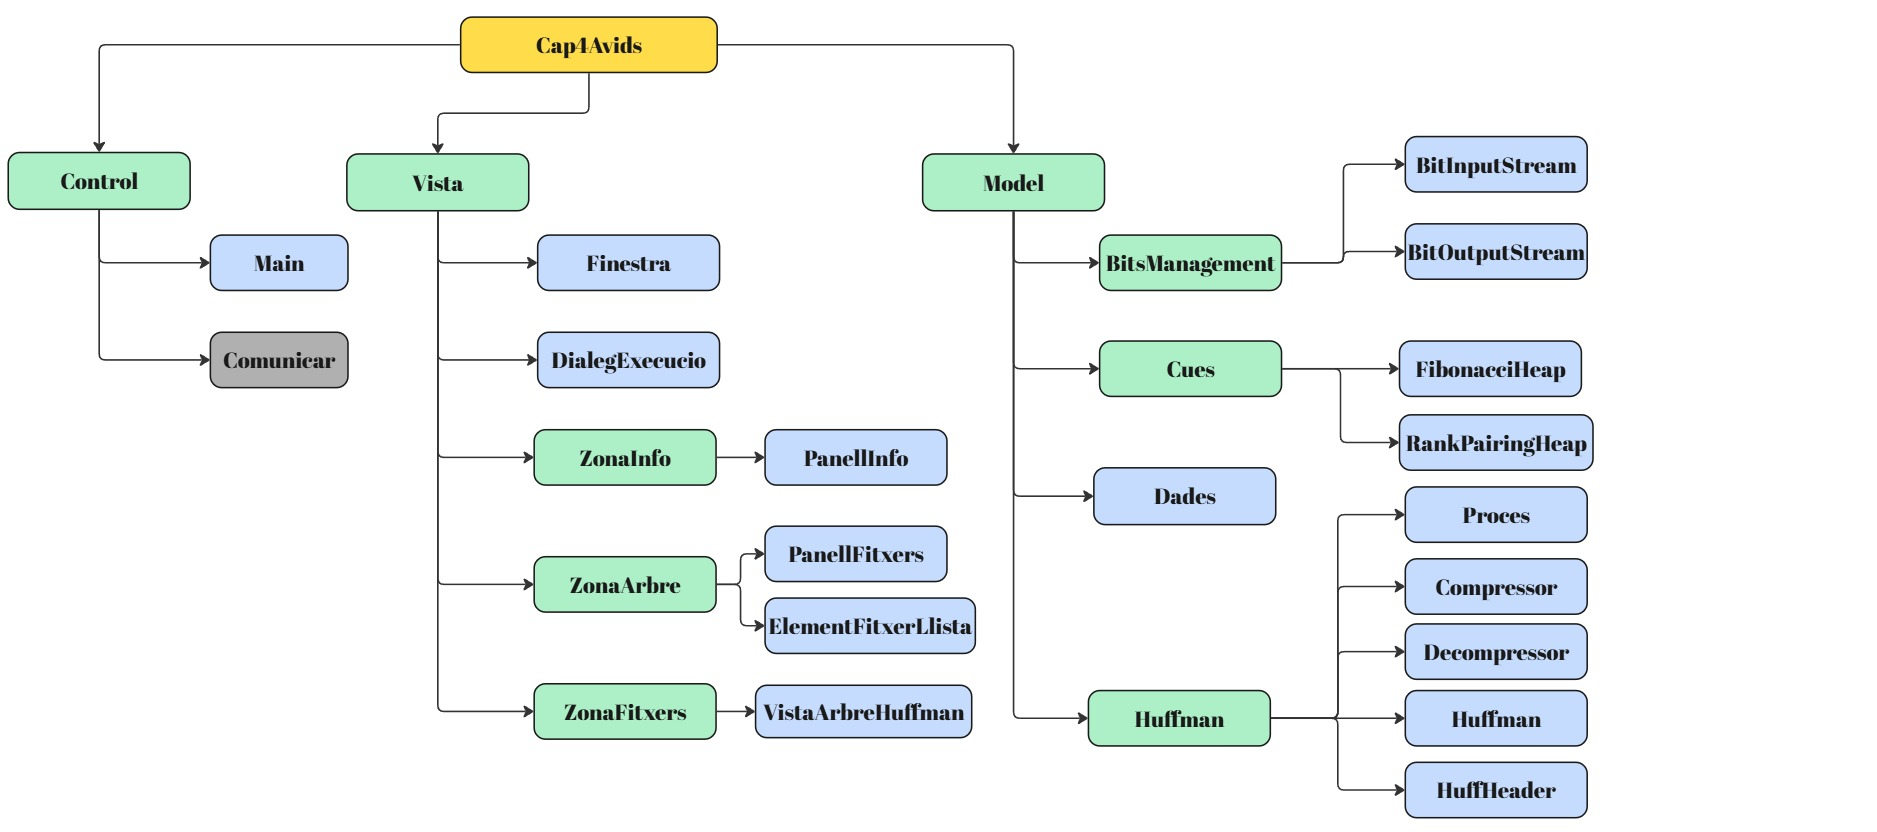
\includegraphics[width=\linewidth, keepaspectratio]{png/estructura.jpg}
    \caption{Estructura de paquets i classes}
    \label{fig:enter-label}
\end{figure}

\subsection{Algorisme de Huffman} 

L’algorisme de Huffman és un \emph{algorisme àvid òptim} que construeix, de baix a dalt, un arbre binari ple seleccionant en cada iteració els dos subarbres de freqüència mínima \cite{huffman1952}. Aquesta construcció permet obtenir una codificació de longitud mínima per a cada símbol del conjunt, maximitzant l'eficiència en la compressió de dades.\newline

El procés comença amb la construcció de la taula de freqüència de símbols, on es recull concurrentment la freqüència d’aparició de cada símbol en l’entrada. A partir d’aquestes freqüències, es construeix iterativament un arbre binari, on els nodes més superiors representen els símbols amb freqüència més alta. \newline

Una vegada es té l'arbre, es genera la taula de codificació mitjançant el recorregut de l'arbre. Durant aquest recorregut, s’assignen valors: 0 als nodes de l’esquerra i 1 als nodes de la dreta, fins a arribar als nodes fulla que representen els símbols de l’alfabet. Aquesta assignació proporciona un codi prefix-free, on cap codi és prefix d’un altre, garantint així la desambiguació durant la descodificació.

\begin{figure}[h]
    \centering
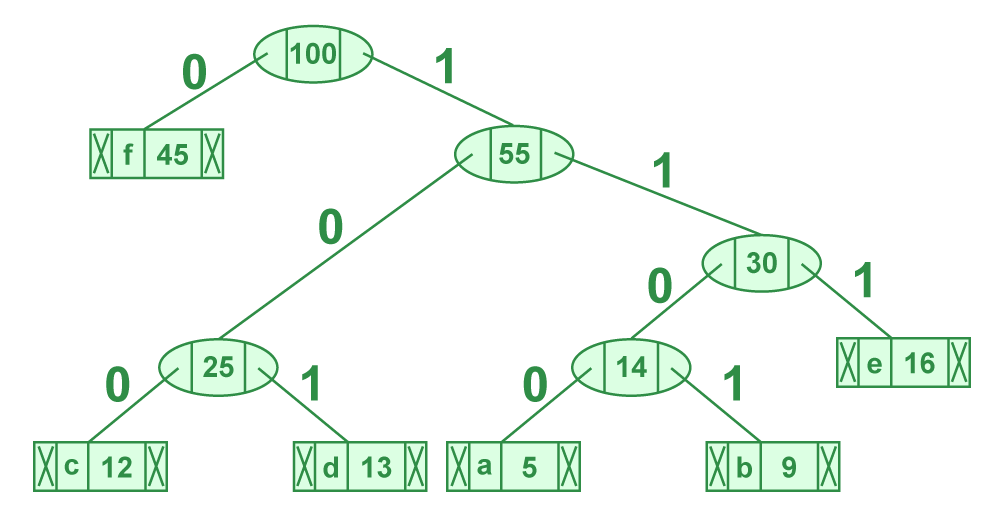
\includegraphics[width=\linewidth]{png/huffman.png}
    \caption{Exemple d'un arbre de Huffman.}
    \label{fig:enter-label}
\end{figure}


El cost temporal de l'algorisme ve dominat pel manteniment de la cua de prioritat $Q$ que conté els pesos dels sub-arbres. La complexitat temporal depèn de l'estructura de dades utilitzada per implementar $Q$. \newline
Si $|C|$ és el nombre de símbols:

\begin{equation}
T_{\text{Huff}}(|C|)=
  \begin{cases}
    \mathcal{O}\!\bigl(|C|\log |C|\bigr)      & \text{Binary Heap},\\[4pt]
    \mathcal{O}\!\bigl(|C|\,\log \log|C|\bigr) & \text{Fibonacci Heap \cite{fredman1987}},\\[4pt]
    \mathcal{O}\!\bigl(|C|\bigr)  & \text{Rank-Pairing Heap \cite{kaplan2013}}.
  \end{cases}
\end{equation}

Nosaltres hem implementat tres variants de $Q$: \textbf{Binary Heap}, \textbf{Fibonacci Heap} i \textbf{Rank-Pairing Heap}; l’usuari pot seleccionar l’estructura preferida des del diàleg de configuració. Aquesta flexibilitat permet avaluar empíricament l’impacte de l’estructura de dades en el temps de compressió, oferint una eina potent per optimitzar el rendiment segons les necessitats específiques del projecte.\newline

Finalment, aquesta classe implementa també el mètode responsable de la generació de les codificacions canòniques que es mostra a la Figura 1 de la secció \textbf{Representació canònica}

\subsection{Header}
La classe \texttt{HuffHeader} encapsula les dades que es guarden a la capçalera dels fitxers comprimits.

Mitjançant atributs com ara els nombres màgics (característics de l'extensió \textbf{.huf} amb què es desen els fitxers comprimits), el nombre de símbols únics (\texttt{uniqueSymbols}), la longitud de l'extensió del fitxer original (\texttt{extensionLength}), etc., es pot representar tota la informació necessària per a la descompressió futura del fitxer, a banda del seu contingut original.\newline

\begin{lstlisting}[language= Java, breaklines = true]
public class HuffHeader {
    public static final int N_CHUNKS = 16;
    public  final byte[] magicN = new byte[magicNumbers.length];
    public byte byteSize;
    public byte extensionLength;
    public byte[] originalExtension;
    public int uniqueSymbols;
    public Map<Long, Integer> codeLengths;
    public Class<? extends Number> mapClass;
    public long originalBytes;
    public int[] bitTamChunks = new int[N_CHUNKS];
\end{lstlisting}
La classe implementa dos mètodes principals, emprats respectivament pel compressor i el descompressor.\newline

El mètode \textit{write} permet guardar la informació en una instància de la classe i escriure-la posteriorment al fitxer comprimit:

\begin{lstlisting}[language = Java, breaklines = true]
public static void write(HuffHeader h, DataOutputStream dos) throws IOException {
    dos.write(h.magicN);
    dos.writeByte(h.byteSize);
    dos.writeByte(h.extensionLength);
    dos.write(h.originalExtension);
    dos.writeInt(h.uniqueSymbols);
    Consumer<Long> call = getWriteConsumer(dos, h);
    for(Map.Entry<Long, Integer> entry : h.codeLengths.entrySet()){
        call.accept(entry.getKey());
        dos.writeInt(entry.getValue());
    }
    dos.writeLong(h.originalBytes);
    for(int o: h.bitTamChunks){
        dos.writeInt(o);
    }
    dos.flush();
    }
\end{lstlisting}

D'altra banda, el mètode \textit{read}, emprat pel descompressor, permet recuperar els atributs de la capçalera del fitxer comprimit i retorna una instància de \texttt{HuffHeader} amb aquesta informació:

\begin{lstlisting}[language = Java, breaklines = true]
public static HuffHeader read(DataInputStream dis) throws IOException {
    HuffHeader h = new HuffHeader();
    dis.readFully(h.magicN);
    if (!Arrays.equals(h.magicN, magicNumbers)) {
        return null;
    }
    h.byteSize = dis.readByte();
    h.extensionLength = dis.readByte();
    h.originalExtension = new byte[h.extensionLength];
    dis.readFully(h.originalExtension);
    h.uniqueSymbols = dis.readInt();
    Callable<? extends Number> call = getReadCallable(dis, h);
    h.codeLengths = new TreeMap<>(Long::compareUnsigned);
    for (int i = 0; i < h.uniqueSymbols; i++) {
        try {
            Number sym =  call.call();
            Integer len = dis.readInt();
            h.codeLengths.put(sym.longValue(), len);
        } catch (Exception e) {
            throw new RuntimeException(e);
        }
    }
    h.originalBytes = dis.readLong();
    for (int i = 0; i < h.bitTamChunks.length; i++) {
        h.bitTamChunks[i] = dis.readInt();
    }
    return h;
    }
\end{lstlisting}

Altres mètodes auxiliars que implementa aquesta classe són \textit{getReadCallable} i \textit{getWriteConsumer}. 

El mètode \textit{getReadCallable} retorna una instància de \texttt{Callable<? extends Number>} que permet llegir, des d’un flux d’entrada, símbols codificats amb el tipus numèric corresponent segons el valor de l’atribut \textbf{byteSize}. Per exemple, si \texttt{byteSize} és 4, es llegiran valors de tipus \texttt{int} mitjançant \texttt{readInt()}. A més, aquest mètode estableix el camp \textit{mapClass} amb la classe del tipus numèric emprat.\newline

D'altra banda, el mètode \textit{getWriteConsumer} retorna un \texttt{Consumer<Long>} que s'encarrega d'escriure valors a un flux de sortida segons el tipus de dada determinat per \texttt{byteSize}. Per exemple, si \texttt{byteSize} és 2, els valors s’escriuen com a \texttt{short} mitjançant \texttt{writeShort()}. Igual que el mètode anterior, també actualitza el camp \texttt{mapClass} amb la classe corresponent. \newline

Pel que fa a la concurrència en aquesta classe, s'ha definit un array d'enters (\textbf{bitTamChunks}) que permet emmagatzemar la mida, en bits, de cada fragment de dades. Aquesta estructura facilita la distribució de la lectura o l'escriptura de dades entre diversos fils d'execució concurrents, ja que cada fil pot treballar amb un fragment (chunk) independent.\newline

Aquests mètodes permeten adaptar dinàmicament la lectura i escriptura dels símbols en funció de la seva mida, optimitzant així l’ús d’espai en la capçalera del fitxer.


\subsection{Mètode de compressió i descompressió}

\paragraph{Classe \texttt{Compressor}} 

La classe \texttt{Compressor} encapsula la lògica per generar un fitxer comprimit a partir d’un arxiu d’entrada. Inicialment, obté la taula de freqüències mitjançant la classe \texttt{Huffman} i en calcula la representació canònica, tal com s’ha descrit a la secció del marc teòric. \newline

Pel que fa a la capçalera del fitxer, aquesta es construeix i escriu emprant el mètode estàtic \texttt{write} de la classe \texttt{HuffHeader}. Aquesta capçalera inclou: els \textit{magic bytes} que identifiquen el format \textbf{.huf}, la mida de símbol (\texttt{byteSize}), la longitud de l’extensió original, l’extensió del fitxer (per exemple, \texttt{.txt}), el nombre de símbols únics i, finalment, la llista canònica de parelles \texttt{(símbol, longitud)} codificada dinàmicament segons el tipus més eficient (byte, short, int o long). També s’hi afegeix la mida original del fitxer en bytes.\newline


Per a la sortida codificada, s’utilitza la classe auxiliar \texttt{BitOutputStream}, que s’encarrega d’encaixar els bits en bytes i aplicar el \textit{padding} necessari per completar l’últim byte del flux. \newline
A més, s'ha implementat un mecanisme de paral·lelització que divideix el flux d’entrada en blocs de mida ajustada automàticament segons el nombre de fils disponibles (\texttt{N\_THREADS}). Cada fil executa la funció de compressió sobre un segment específic del flux mitjançant crides a la funció \textit{comprimir()}, i es sincronitzen posteriorment amb \textit{waitAll()}. Els resultats parcials es guarden en \texttt{fileChunks} i es fusionen a la sortida final. Finalment, el vector \texttt{bitTamChunks} s’assigna amb les mides (en bits) de cada bloc processat, de manera que permet reconstruir correctament el flux durant la descompressió.
\begin{lstlisting}[language = Java, breaklines = true]
    //.. codi del header..
  //Escriure la codificacio del contingut de l'arxiu d'entrada
try (InputStream fis = new BufferedInputStream(Files.newInputStream(inputPath))) {
    byte[] bfis = fis.readAllBytes();
    int split = Math.max(((bfis.length/huffH.byteSize) / N_THREADS)*huffH.byteSize, 256);
    //System.err.println("C: split = " + split + ", bytes = " + bfis.length + ", " + (split*N_THREADS));
    for (int i = 0; i < N_THREADS - 1 && i * split < bfis.length; i++) {
        int finalI = i;
        executar(() -> {
            comprimir(finalI, bfis, finalI*split, (finalI+1)*split, canonCodes, huffH.byteSize);
        });
    }
    executar(()-> {
        comprimir(N_THREADS-1, bfis, (N_THREADS-1) * split, bfis.length, canonCodes, huffH.byteSize);
    });
    waitAll();

    huffH.bitTamChunks = chunksSizes;
    HuffHeader.write(huffH, dos);
    dos.flush();
    for(ByteArrayOutputStream fileChunk : fileChunks) {
        if(fileChunk == null) {
            continue;
        }
        fileChunk.writeTo(bufOut);
    }
}    
\end{lstlisting}

El mètode \texttt{comprimir} s’encarrega de processar un fragment del bloc de dades original (\texttt{arr}) comprenent les posicions entre \texttt{ini} i \texttt{fi}, i codificar-lo utilitzant els codis de Huffman canònics (\texttt{canonCodes}). Per a cada símbol del fragment, s’agrupen \texttt{byteSize} bytes consecutius per formar una única entitat de tipus \texttt{long}, que s’utilitza com a clau per obtenir el codi Huffman corresponent. Aquest codi, representat com un array de bits, s’escriu,de bit a bit, al flux \texttt{BitOutputStream}. Un cop completat el procés, s’actualitza el vector \texttt{chunksSizes} amb la mida en bits del fragment comprimit i es desa el resultat parcial al vector \texttt{fileChunks}.

\begin{lstlisting}[language = Java, breaklines = true]      
try (ByteArrayOutputStream bos = new ByteArrayOutputStream(Math.max(fi - ini, 0));
             BitOutputStream bos2 = new BitOutputStream(bos)) {
        for (int i = ini; i < arr.length && i < fi; i += byteSize) {
            long b = (long) arr[i] & (0xFFL);
            for (int j = 1; j < byteSize; j++) {
                b <<= 8;
                int aux;
                if ((i + j) >= arr.length)
                    aux = 0;
                else {
                    aux = arr[i + j];
                }
                b |= (long) aux & (0xFFL);
            }
            byte[] codeBits = canonCodes.get(b);
            assert codeBits != null;
            for (byte codeBit : codeBits) {
                bos2.writeBit(codeBit == 1);
            }
        }
        chunksSizes[id] = bos2.size();
        bos2.flush();
        fileChunks[id] = bos;
    } catch (IOException e) {
        throw new RuntimeException(e);
    }
}
\end{lstlisting}
\paragraph{Classe \texttt{Decompressor}}  
La classe \texttt{Decompressor} s'encarrega de reconstruir el contingut original a partir del fitxer comprimit. Primer, fa ús del mètode estàtic \texttt{read} de la classe \texttt{HuffHeader}, que llegeix tots els atributs de la capçalera en el mateix ordre en què van ser escrits: els \textit{magic bytes} (identificadors del format), la mida de símbol utilitzada (\textit{byteSize}), la longitud i l’extensió del fitxer original, el nombre total de símbols únics, la llista canònica de parelles \textit{(símbol, longitud)} i, finalment, la mida original del contingut en bytes i els tamanys en bits de cada fragment codificat (\texttt{bitTamChunks}).

Amb la informació obtinguda, es reconstrueix la representació canònica dels codis Huffman mitjançant \texttt{Huffman.generateCanonicalCodes(codeLengths, symbols)} i es construeix l’arbre de descodificació amb el mètode \texttt{buildDecodingTree()}, que recorre cada seqüència binària per assignar símbols (0 per anar a l’esquerra, 1 per anar a la dreta) a les seves respectives fulles.

\begin{lstlisting}[language= Java, breaklines = true]
 private DecodeNode buildDecodingTree(Map<Long, byte[]> codes) {
    DecodeNode root = new DecodeNode();
    for (Map.Entry<Long, byte[]> entry : codes.entrySet()) {
        byte[] code = entry.getValue();
        if (code == null) continue;
        DecodeNode node = root;
        for (byte c : code) {
            if (c == 0) {
                if (node.left == null) node.left = new DecodeNode();
                node = node.left;
            } else {
                if (node.right == null) node.right = new DecodeNode();
                node = node.right;
            }
        }
        node.symbol = entry.getKey();
    }
    return root;
}
\end{lstlisting}

A continuació, es divideix el flux codificat en fragments segons els valors emmagatzemats a \texttt{bitTamChunks}. Cada fragment es processa en paral·lel amb diversos fils mitjançant el mètode \texttt{decode()}, el qual recorre l’arbre de descodificació bit a bit fins a recuperar el símbol original. Aquest símbol es reconstrueix amb el nombre de bytes adequat (\texttt{byteSize}) i s'escriu en un \texttt{ByteArrayOutputStream} individual per a cada fil. Un cop tots els fils han acabat, els fragments resultants es concatenen i s'escriuen al fitxer de sortida. Finalment, es calcula el temps total de descompressió i es registra amb la resta de dades estadístiques. \newline

\begin{lstlisting}[language= Java, breaklines = true]
private void decode(int id, byte[] arr, int ini, DecodeNode root, int bitCap, int byteSize) {
    ByteArrayOutputStream bos = new ByteArrayOutputStream();
    try (ByteArrayInputStream bais = new ByteArrayInputStream(arr);
         BitInputStream bis = new BitInputStream(bais)) {
        bais.skip(ini);
        int read = 0;
        while (read < bitCap) {
            DecodeNode node = root;
            while (!node.isLeaf() && read < bitCap) {
                boolean bit = bis.readBit();
                read++;
                node = bit ? node.right : node.left;
            }

            long aux = node.symbol;
            for (int i = 0; i < byteSize; i++) {
                int bits = (int) ((aux & (0xFFL << (8 * (byteSize - i - 1)))) >> (8 * (byteSize - i - 1)));
                bos.write(bits);
            }
        }
    } catch (IOException e) {
        throw new RuntimeException(e);
    } finally {
        fileChunks[id] = bos;
    }
}    
\end{lstlisting}

Amb aquest parell de classes s’aconsegueix una solució completa per a comprimir i descomprimir qualsevol fitxer , aprofitant l’eficiència de l’algorisme de Huffman i la codificació canònica per reduir l’espai i accelerar la generació i interpretació dels codis, i l'ús adequat de la concurrència.

\subsection{Cues}

\paragraph{Classe \texttt{FibonnaciHeap}}  
Aquesta classe implementa una estructura de Fibonnaci basada en monticle. Es tracta d'una col·lecció d'arbres que satisfan la propietat de monticle mínim, és a dir, la clau d'un fill sempre és més gran o igual que la clau del pare. Això implica que la clau mínima sempre es troba a l'arrel d'un dels arbres, facilitant així obtenir els nodes mínims de l'estructura.\newline

A nivell d'implementació, utilitza nodes doblement enllaçats i organitzats circularment per afavorir operacions eficients com \texttt{offer}, \texttt{poll} i \texttt{peek}. \newline
Cada \texttt{Node} conté informació sobre el seu element, el seu grau (nombre de fills), una variable booleana per inidcar si està marcat, i referències als seus veïns, fills i pare. \newline

El mètode \texttt{offer} permet inserir nous elements fusionant-los amb el heap existent, mentre que \texttt{poll} elimina el mínim reorganitzant l'estructura amb \texttt{consolidate} per evitar graus duplicats. Les operacions de fusió es fan mitjançant el mètode \texttt{merge}, i les reestructuracions d'arbre amb \texttt{link} i \texttt{delink}. L'estructura afavoreix costos amortitzats baixos i una gestió eficient dels elements.
\begin{figure}[H]
    \centering
    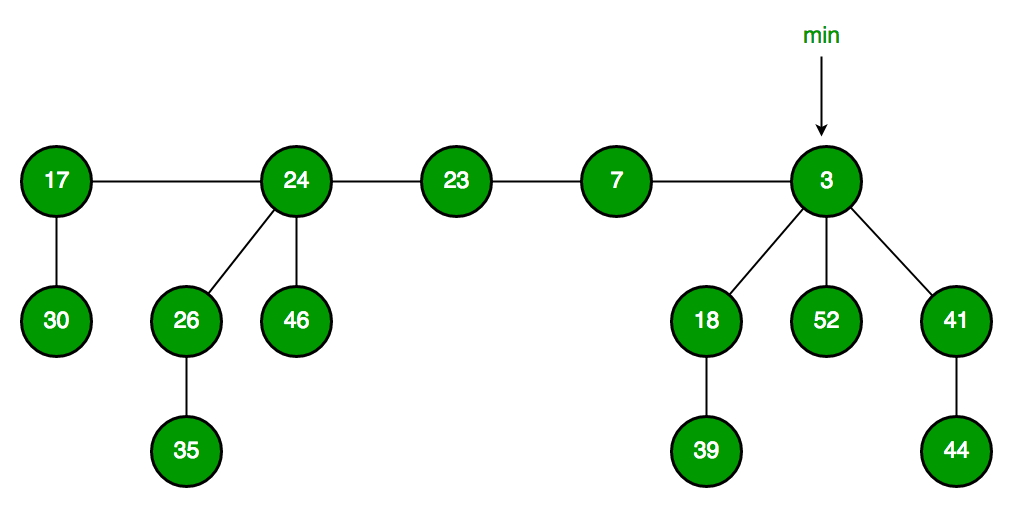
\includegraphics[width=0.5\linewidth]{png/Fibonacci-Heap.png}
    \caption{Exemple del monticle de Fibonnaci}
    \label{fig:enter-label}
\end{figure}


\paragraph{Classe \texttt{RankPairingHeap}}  
La classe \texttt{RankPairingHeap<E>} implementa una cua de prioritat basada en arbres jeràrquics, utilitzant l'estructura de \textit{rank pairing heap}. 
La cua esta formada per  una llista d'arrels , instàncies de la classe \texttt{Node}, que representen arbres independents.
Cada arrel guarda amb un camp \texttt{key}, el seu primer fill, i els germans enllaçats.\newline 

Per insertar un element a la cua, usant el mètode  \texttt{offer}, es crea un nou node i s’afegeix a la llista d’arrels, actualitzant el mínim global (\textit{minRoot}) si cal. \newline 

L’operació \texttt{poll}, per altra banda,  elimina l’arrel amb el valor mínim, afegeix els seus fills a la llista d’arrels, i reorganitza l’estructura mitjançant el mètode \texttt{consolidate}. Aquesta reestructuració agrupa arbres de mateix rang combinant-los amb \texttt{link}, que garanteix que el node amb la clau més petita esdevingui l’arrel del nou arbre, així com  actualitzar el  \texttt{minRoot}. \newline 

Aquesta estructura afavoreix l’eficiència en les operacions d’inserció i extracció mitjançant un sistema de rangs senzill i flexible.


\subsection{Gestió de concurrència}

Respecte a la concurrència, s'ha optat per utilitzar un \texttt{ThreadPoolExecutor}, que permet una gestió eficient dels fils mitjançant un conjunt fix de recursos reutilitzables. Aquesta elecció facilita l'accés a informació rellevant com el nombre de fils actius, el nombre de tasques completades o el nombre de tasques pendents. Així mateix, ha estat possible sotmetre tasques de forma paral·lela, millorant significativament el rendiment en operacions costoses com el càlcul de freqüències dels símbols (implementat a la classe \texttt{Huffman}), i la construcció de la taula de codificació, a més de la compressió i descompressió dels fitxers. Aquesta aproximació permet distribuir la càrrega de treball entre diversos fils, aprofitant millor els recursos de maquinari disponibles i reduint el temps d'execució en fitxers de mida considerable.


\begin{figure}[H]
    \centering
\begin{lstlisting}[language=Java, basicstyle=\ttfamily\small]
private void calculateFreqs() {
    int split = fileBytes.length / N_THREADS;
    for (int i = 0; i < N_THREADS - 1 && split > 0; i++) {
        int j = i;
        addConcurrent(() -> {            recursiveAccumulate(j, j * split, (j + 1) * split);
            });
        }
    //assegurar-se final
    addConcurrent(() -> {            recursiveAccumulate(N_THREADS - 1, (N_THREADS - 1) * split, fileBytes.length);
        });

        //esperar
   joinAll();
   long total = 0;
   for (int i = 0; i < N_THREADS; i++) {
        for (int j = 0; j < freqs.length; j++) {
            freqs[j] += acumulators[i][j];
            total += acumulators[i][j];
        }
    }
   //calcular entropia
   entropia = 0;
   for(long i: freqs) {
        if (i==0) continue;
        double freq =  i / (double) total;
        entropia += freq * Math.log10(freq)/Math.log10(2);
    }
    entropia = -entropia;
}
    \end{lstlisting}
    \caption{Ús de concurrència per al càcul de les freqüències dels símbols.}
\end{figure}


\subsection{Visualització i interacció amb l'usuari}

La interfície gràfica d’usuari (GUI) s’ha desenvolupat amb la llibreria \texttt{Swing} i ha estat dissenyada per oferir una interacció senzilla, intuïtiva i funcional amb el compressor Huffman.

\paragraph{Estructura principal de la finestra}

La finestra principal (\texttt{Finestra}) està organitzada en dues zones clarament diferenciades:
\begin{itemize}
    \item \textbf{Barra d’eines superior}: conté botons per a les accions bàsiques: \emph{Carregar}, \emph{Comprimir}, \emph{Descomprimir} i \emph{Mostrar Arbre}. Cada botó està associat a un \emph{listener} que desencadena una acció concreta mitjançant missatges enviats al controlador principal.
    
    \item \textbf{Àrea de fitxers}: es divideix en dos panells laterals (\texttt{PanellFitxers}):
    \begin{itemize}
        \item \textbf{Arxius a comprimir}: permet afegir fitxers nous a comprimir arrossegant-los directament o seleccionant-los via diàleg de fitxers (\texttt{JFileChooser}).
        \item \textbf{Arxius a descomprimir}: mostra els fitxers ja comprimits (\texttt{*.huf}), i permet seleccionar-los per a descompressió.
    \end{itemize}
\end{itemize}

Els panells de fitxers suporten operacions de \emph{drag \& drop}, així com botons addicionals per afegir, eliminar o netejar els llistats.

\paragraph{Procés de compressió i configuració}

Quan l'usuari prem el botó \emph{Comprimir}, s'obre un diàleg modal (\texttt{DialegExecucio}) que permet configurar paràmetres abans d'executar l'operació:
\begin{itemize}
    \item \textbf{Selecció d'estructura de cua}: triar entre \emph{Binary Heap}, \emph{Fibonnaci Heap} o \emph{Rank-Pairing Heap}.
    \item \textbf{Selecció de mida de paraula}: 8, 16, 32 o 64 bits.
    \item \textbf{Carpeta de destí}: especificació del directori on es desarà el fitxer comprimit.
\end{itemize}
El diàleg genera un missatge de configuració que es comunica al controlador, que inicia el procés de compressió amb els paràmetres seleccionats.
\begin{figure}[H]
    \centering
    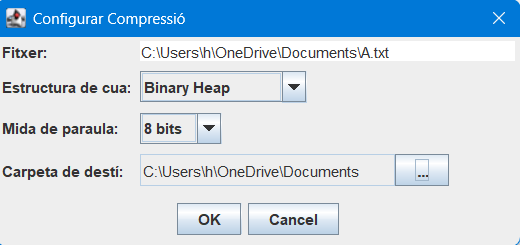
\includegraphics[width=0.5\linewidth]{png/Fcompressio.png}
    \caption{Finestra dels paràmetres de compressió}
    \label{fig:enter-label}
\end{figure}

\paragraph{Procés de descompressió}

De manera similar, en prémer \emph{Descomprimir}, s'obre un diàleg (\texttt{DialegExecucio}) adaptat per a la descompressió, sol·licitant únicament la carpeta de destí per guardar els fitxers restaurats.
\begin{figure}[H]
    \centering
    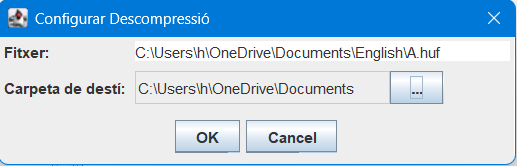
\includegraphics[width=0.5\linewidth]{png/fDecompressio.png}
    \caption{Finestra dels paràmetres de decompressió}
    \label{fig:enter-label}
\end{figure}

\paragraph{Acció \emph{Mostrar Arbre}}

Seleccionant un fitxer comprimit i prement \emph{Mostrar Arbre}, es mostra l'arbre de codificació de huffma
\begin{figure}[H]
    \centering
    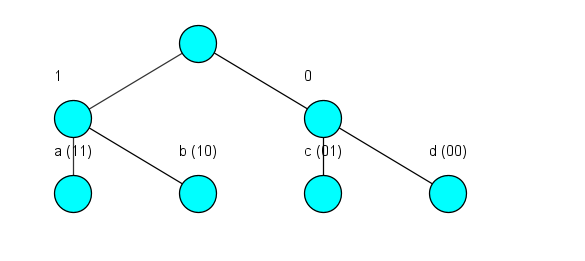
\includegraphics[width=0.5\linewidth]{png/arbre.png}
    \caption{Arbre de huffman}
    \label{fig:enter-label}
\end{figure}
\vspace{1em}

\paragraph{Panell d'informació}
De manera opcional s'ha afegit un panell a la finestra del programa que permet visualitzar les dades o estadístiques dels processo de compressió i decompressió. 

\begin{figure}[H]
    \centering
    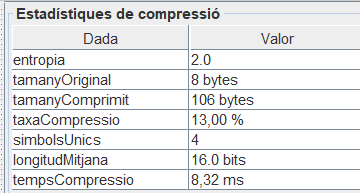
\includegraphics[width=0.5\linewidth]{png/estdCompressio.png}
    \caption{Exemple d'estadístiques de compressió}
    \label{fig:enter-label}
\end{figure}

\begin{figure}[H]
    \centering
    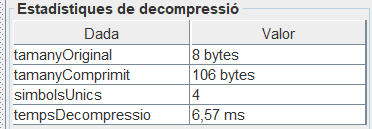
\includegraphics[width=0.5\linewidth]{png/estdDecompressio.png}
    \caption{Exemple d'estadístiques de decompressió}
    \label{fig:enter-label}
\end{figure}

La interfície gràfica resultant combina simplicitat d'ús amb flexibilitat operativa, facilitant tant les operacions bàsiques de compressió i descompressió com la configuració de paràmetres avançats.


\subsection{Decisions de disseny i extres implentats}

Pel que fa a les millores implementades, hem incorporat dues cues prioritàries addicionals: el monticle de Fibonacci i el monticle de Rank Pairing, que ofereixen costos amortitzats optimitzats. A més, s'ha afegit una funcionalitat que calcula i mostra, mitjançant una finestra, el temps que tarden els processos principals del programa, com ara la compressió i la descompressió d'arxius, finalment, s'ha afegit l'opció de triar varis tamanys de paraula en la compressió.

Adicionalment, s'ha afegit la funcionalitat de visualitzar l'arbre de huffman a partir d'un fitxer comprimit.



\section{Arquitectura del Programa}

L’aplicació segueix una arquitectura basada en el patró Model-Vista-Controlador (MVC), que separa clarament la lògica de negoci, la interfície gràfica i el flux de control. Aquest enfocament facilita tant la mantenibilitat del codi com la seva extensibilitat futura.\newline

El \textbf{model} encapsula les estructures de dades i la lògica algorísmica associada a la generació dels arbres de huffman, el càlcul de les freqüències, la compressió i decompressió dels arxius, la implementació de diferents cues per als arbres de huffman, entre altres coses.

La \textbf{vista} proporciona una representació gràfica intuïtiva de dos panells principals per poder carregar fitxers per a la compressió o decompressió.

\begin{figure}[h]
    \centering
    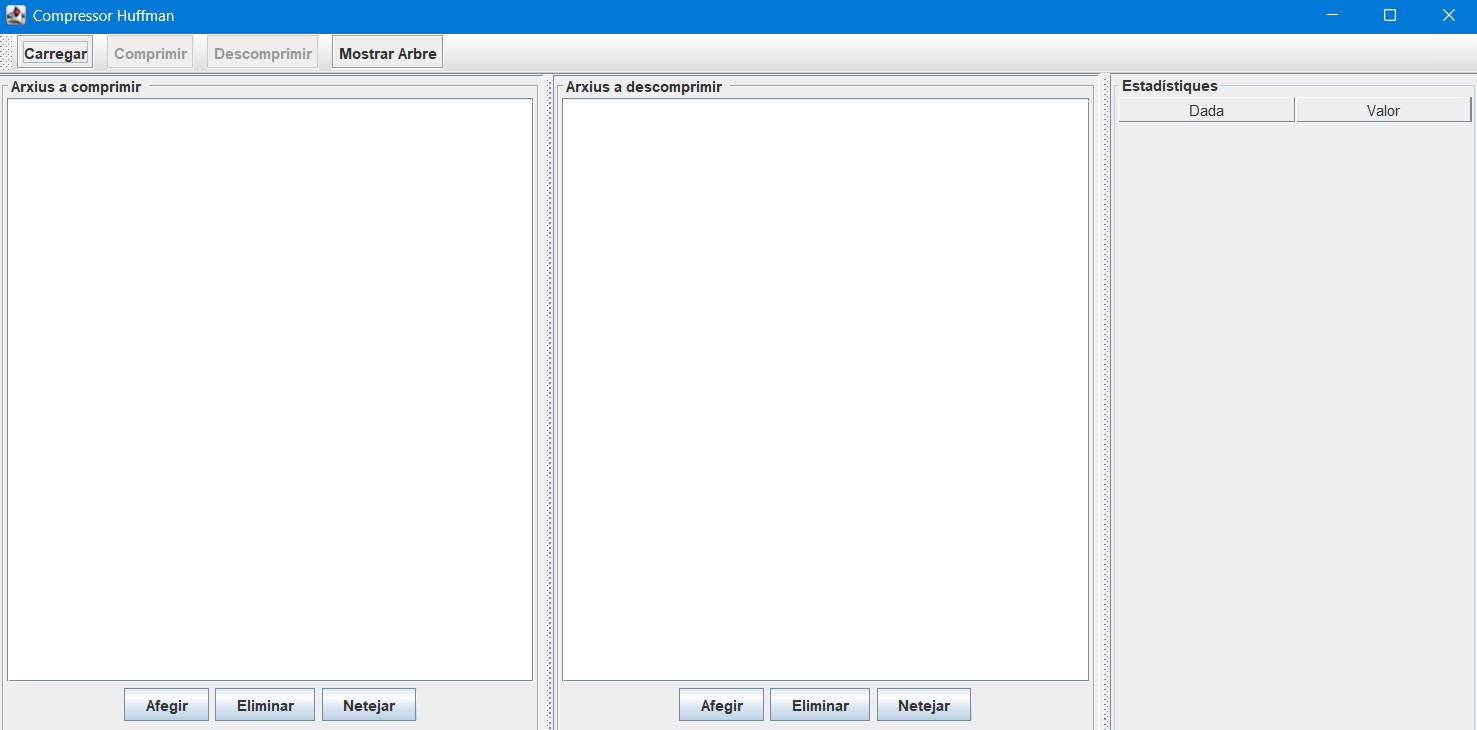
\includegraphics[width=\linewidth]{png/vista.png}
    \caption{Finestra principal del programa}
    \label{fig:enter-label}
\end{figure}

El \textbf{controlador}, integrat principalment a la classe \texttt{Main}, gestiona el flux d’execució i la comunicació entre el model i la vista. La comunicació entre components es basa en una interfície comuna (\texttt{Comunicar}), que garanteix la modularitat i redueix la dependència entre mòduls.

Aquesta arquitectura modular facilita l’evolució del sistema, per exemple permetent incorporar noves estratègies de càlcul o nous tipus de visualització sense afectar els altres components.



\section{Resultats i Comparació}
En aquesta secció s'analitza el rendiment de l'aplicació a partir d'experiments sistemàtics. D'una banda, es comparen les diferents implementacions de monticles (PriorityQueue, Fibonacci Heap i Rank Pairing Heap) en termes de temps d'execució i ús de memòria durant la construcció de l'arbre de Huffman; d'altra banda, s'examina la taxa de compressió obtinguda amb fitxers d'entrada de tamany incremental.\newline

Per dur a terme els experiments s'han generat fitxers de prova mitjançant una eina de generació de text aleatori (Lorem Ipsum \cite{LoremIpsum}).


\begin{table}[H]
    \centering
    \begin{tabular}{|l|l|l|l|}
        \hline
        \textbf {N} & \textbf{PriortyQueue} & \textbf{Fibonnaci Heap} & \textbf{Rank Pairing Heap} \\
        \hline
         1KB &	  7750700   &	 5056600  &   3958200 \\
        10 KB &	   7012100  &	  4280500  &   3409100 \\
        100KB &   10220800  &	 11464500  &   3131500 \\
        1MB	&     13679500  &    21435300  &   15778700 \\
        10MB &	  75881300  &	 71784900  &  69371700 \\
        100MB &	 615597100  &   562691100 &	 582138400 \\
        500MB & 7102013700  &  2900767800 &	2763970200\\
        1000MB&	6196001100	&  5728621700 &	5515223100\\
        \hline
    \end{tabular}
    \vspace{3mm}
    \caption{Temps d'execució (ns) de l'algorisme de Huffman en funció de diferentes implementacions de monticles}
    \label{tab:complexitat}
\end{table}

\begin{table}[H]
    \centering
    \begin{tabular}{|l|l|l|l|}
        \hline
        \textbf {N} & \textbf{PriortyQueue} & \textbf{Fibonnaci } & \textbf{Rank Pairing } \\
        \hline
         1KB	 &22179	&7653	&5867\\
        10 KB	&5459	&5864	&5412\\
        100KB	&7246	&7293	&7217\\
        1MB	    &11694	&34654&	17227\\
        10MB	&99311&	107007	&125803\\
        100MB	&443814&	318887&	367785\\
        500MB	&1451808&	823414	&733282\\
        1000MB	&2569888	&1641739&	2310469\\
                \hline
    \end{tabular}
    \vspace{3mm}
    \caption{Memòria usada (en KB) per a la construcción de l'arbre de huffman per a diferentes implementacions de monticles}
\end{table}

\begin{table}[H]
    \centering
    \begin{tabular}{|l|l|l|}
        \hline
        \textbf {Tamany d'arxiu (B)} & \textbf{Tamany comprimit (B)} & \textbf{\% Compressió} \\
        \hline
        1024       &	 820  &  19,92\\
        10240      &	5798 &   43,38\\
        102400     &	55266 & 46,03\\
        1048576    &	563077 & 46,30\\
        10485760   &	5627997 & 46,33\\
        104857600  &	56277390 & 46.33\\
        524288000  &	281385742 &  46,33\\
        1073741824 &	576277674 &  46,33\\
        \hline
    \end{tabular}
    \vspace{3mm}
    \caption{Tamany de fitxers comprimits per a diferentes mides d'arxius d'entrada.}
\end{table}

\begin{table}[H]
    \centering
    \begin{tabular}{|l|l|l|}
        \hline
        \textbf {Tamany d'arxiu (B)} & \textbf{T. compressió (ns)} & \textbf{T. descompressió (ns)} \\
        \hline
        1024       &	35576100 & 6800000\\
        10240      &	4649100 &   5323400\\
        102400     &	62044800 & 58846800\\
        1048576    &	78585400 & 13644900\\
        10485760   &	197526900 & 72601700\\
        104857600  &	359548000 & 463239400\\
        524288000  &	2316985000 &  7620941900\\
        1073741824 &	14106173400 &  18934915900\\
        \hline
    \end{tabular}
    \caption{Temps d'execució per a diferentes mides d'arxius d'entrada.}
\end{table}

\begin{table}[H]
    \centering
    \begin{tabular}{|l|l|l|}
        \hline
        \textbf {Tamany de paraula} & \textbf{Temps (ns)} & \textbf{Tamany (B)} \\
        \hline
        8 bits       &	327959100 & 56277390 \\
        16 bits     &	487414300 &   49470775\\
        32 bits     &	372045000 & 35790924\\
        64 bits    &	636928900 & 24031712\\

        \hline
    \end{tabular}
    \caption{Temps d'execució per a diferents tamanys de paraula per l'arxiu de 100MB.}
\end{table}

De forma visual, obtenim les següents gràfiques respectivament.

\begin{figure}[H]
    \centering
    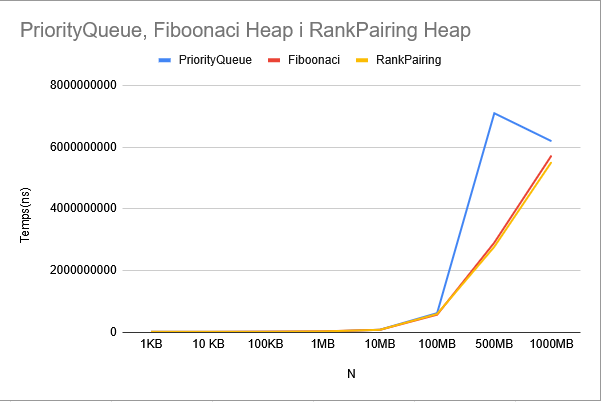
\includegraphics[width=1\linewidth]{png/three queues appear at Memorias edge.png}
    \caption{Temps de contrucció de l'arbre de huffman per differents monticles}
    \label{fig:enter-label}
\end{figure}

\begin{figure}[H]
    \centering
    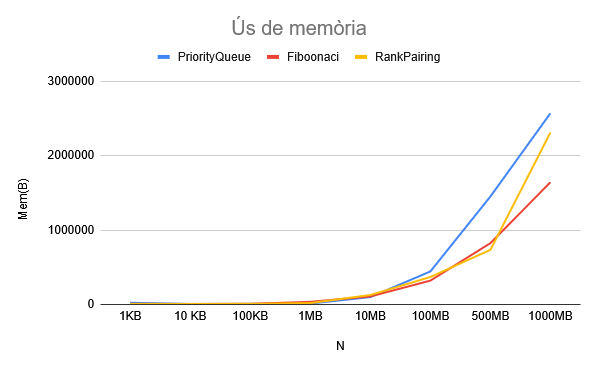
\includegraphics[width=1\linewidth]{png/neo_us_memoria.png}
    \caption{Ús de memòria segons el tipus de monticle}
    \label{fig:enter-label}
\end{figure}
\begin{figure}[H]
    \centering
    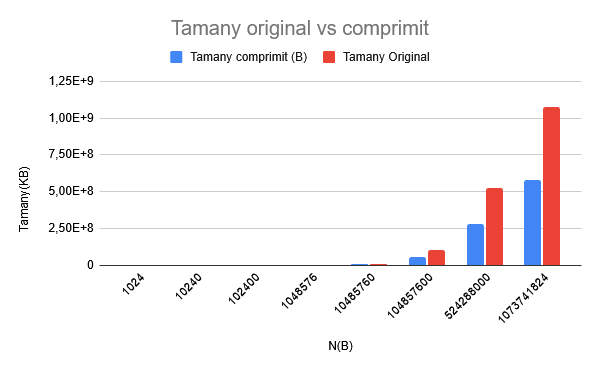
\includegraphics[width=1\linewidth]{png/neo_comparativa_tamanys.png}
    \caption{Taxa de compressió de l'algorisme de huffman}
    \label{fig:enter-label}
\end{figure}



Els resultats experimentals indiquen clarament que la implementació amb PriorityQueue és relativament inferior: en gairebé tots els casos el temps d'execució és superior al dels altres mètodes, especialment amb fitxers de mida elevada (a partir de 500MB), tot i que en arxius de mida petita (10KB) es poden observar lleugeres variacions. D'altra banda, el Fibonacci Heap sol oferir un rendiment lleugerament similar al del Rank Pairing Heap en alguns casos, encara que aquest últim mostra unes creixents d'ús de memòria elevats a partir de 500MB.\newline

Pel que fa a l'ús de memòria, tant PriorityQueue com Fibonacci mostren un creixement moderat del consum de memòria segons el tamany del fitxer, que RankPairing manté, però a partir de 500MB aquest es dispara. \newline

Aquest comportament es pot atribuir a les diferències en la implementació interna de cada estructura. Mentre que el PriorityQueue es basa en un heap binari senzill, amb overhead mínim, tant el Fibonacci Heap com el Rank Pairing Heap, tot i oferir avantatges teòrics (per exemple, insercions en temps constant de manera amortitzada), introdueixen complexitat addicional en la consolidació dels nodes, que segons l'ús de la cua pot resultar beneficiós. 

\begin{table}[h]
    \centering
    \begin{tabular}{|l|l|l|l|}
        \hline
        \textbf{Operació} & \textbf{PriorityQueue} & \textbf{Fibonacci*} & \textbf{RankPairing*} \\
        \hline
        offer      & \( O(\log N) \) & \( O(1) \) & \( O(\log N) \) \\
        poll       & \( O(\log N) \) & \( O(\log N) \) & \( O(\log N) \) \\
        peek       & \( O(1) \) & \( O(1) \) & \( O(1) \) \\
        consolidate & — & \( O(\log N) \) & \( O(\log N) \) \\
        \hline
    \end{tabular}
     \vspace{2mm}
    \caption{Costs computacionals de les operacions en diferents monticles (* Indica un cost amortitzat).}

\end{table}


Quant a la taxa de compressió, es pot observar que a mesura que augmenta el tamany de l'arxiu d'entrada, la compressió es torna més eficient. Aquest fenomen s'explica per la major amortització de les dades de capçalera sobre fitxers amb un volum de dades considerable, resultant en una reducció percentual del tamany comprimit.\newline

Segons el tamany de paraula triat a l'hora de comprimir, tant el temps com el tamany de l'arxiu comprimit varia. En aquest cas, amb un arxiu de lorem es pot apreciar que al augmentar el tamany de paraula, el temps de compressió augmenta, però el tamany resultant es menor, passant d'una compressió d'un 46,33\% amb 8 bits a un 77,08\%.\newline

En conclusió, els experiments confirmen que, per al nostre cas d'ús (construcció de l'arbre de Huffman i compressió de fitxers), la implementació basada en Fibonacci és la més recomanable, ja que ofereix un excel·lent equilibri entre rendiment temporal i ús de memòria. Cada implementació té els seus avantatges teòrics, però en l'aplicació pràctica aquests resultats experimentals recolzen clarament el Fibonacci com la millor opció.

\section{Conclusions}

A nivell global, tenim una valoració positiva del treball realitzat, tot i que som conscients que podríem haver implementat més funcionalitats addicionals. Aquesta observació, però, sempre serà certa, ja que qualsevol projecte podria expandir-se amb més característiques si es disposa de més temps o recursos.\newline

L'abundància de recursos disponibles sobre l'algorisme de Huffman i els processos de compressió i descompressió ens ha estat de gran ajuda. Aquesta informació ens ha proporcionat una base sòlida i una comprensió clara per definir l'estructura general del nostre programa. A més, cal destacar que tots els membres de l'equip ja havien treballat amb una pràctica de grau relacionada amb la implementació de l'algorisme de Huffman, fet que ha facilitat la nostra tasca.\newline

Pel que fa a les implementacions, ens ha sorprès el millor rendiment, en general, de les nostres implementacions de Fibonacci i el Rank Pairing, ja que pensaven que una estructura de dades integrada en les llibreries estàndard de Java destacaria per sobre les altres. En qualsevol cas, aquesta pràctica ha complert amb el seu objectiu principal: comparar el rendiment de diversos monticles i determinar quines són les situacions òptimes per utilitzar cada un d'ells.\newline

D'altra banda, la introducció de concurrència ha demostrat ser un gran avenç, especialment quan hem treballat amb arxius d'entrada de tamany considerablement gran. Això ha suposat una millora notable en el rendiment del programa. No obstant això, també s'ha tingut en compte que la concurrència introdueix una certa càrrega addicional per a la coordinació i sincronització entre threads, per això s'ha establert un mínim de tamany a partir del qual es pot optar per l'ús de la concurrència.\newline

Pel que fa al repartiment de tasques, la figura següent il·lustra com hem organitzat el treball. Tal com fem habitualment, ens hem assegurat que cada part o bloc del projecte fos treballat per dues persones per fomentar la col·laboració i garantir que tothom tingui l'oportunitat de participar en diverses tasques. Aquest enfocament també ha assegurat una distribució equitativa de les responsabilitats i un coneixement compartit dins de l'equip.


\begin{figure}[H]
    \centering
    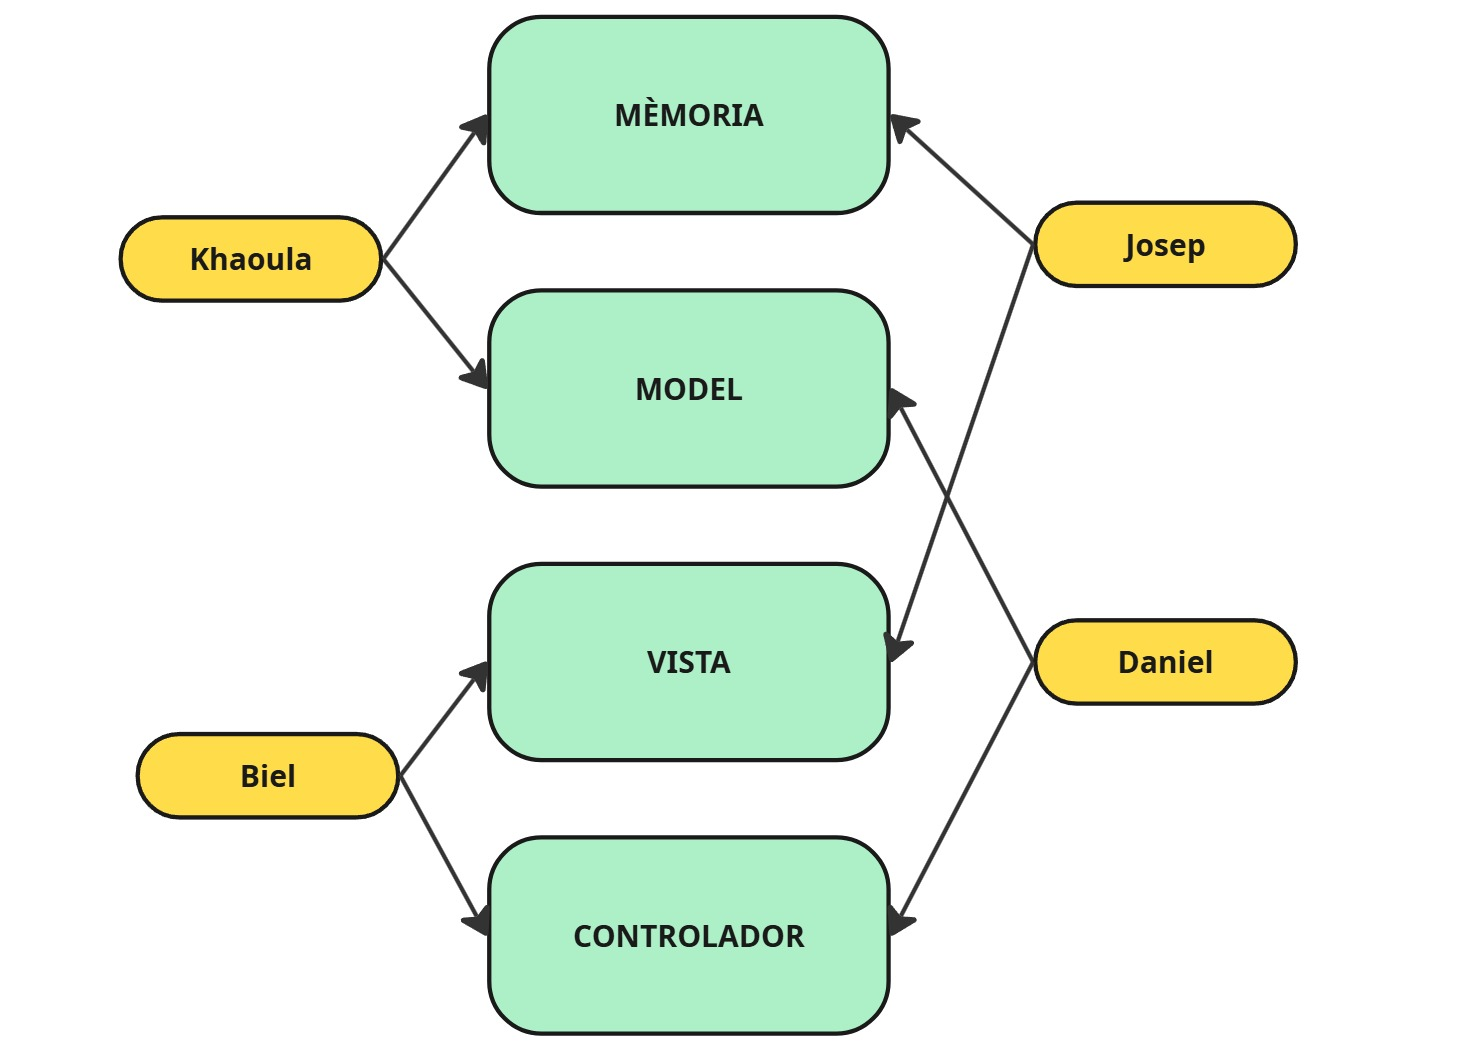
\includegraphics[width=0.75\linewidth]{png/repartimentFeina.jpg}
    \caption{Repartiment de tasques}
    \label{fig:enter-label}
\end{figure}

\bibliographystyle{plain}
\begin{thebibliography}{9}

\bibitem{shannon1948}
C.~E. Shannon.
\newblock A mathematical theory of communication.
\newblock \emph{Bell System Technical Journal}, 27(3):379–423, 1948.

\bibitem{huffman1952}
D.~A. Huffman.
\newblock A method for the construction of minimum‐redundancy codes.
\newblock \emph{Proceedings of the IRE}, 40(9):1098–1101, 1952.

\bibitem{amortized}
GeeksforGeeks.
\newblock Introduction to Amortized Analysis.
\newblock \emph{GeeksforGeeks}, 2019.
\newblock \url{https://www.geeksforgeeks.org/introduction-to-amortized-analysis/}.

\bibitem{fredman1987}
M.~L. Fredman and R.~E. Tarjan.
\newblock Fibonacci heaps and their uses in improved network optimization algorithms.
\newblock \emph{Journal of the ACM}, 34(3):596–615, 1987.

\bibitem{kaplan2013}
H.~Kaplan, N.~Shafrir, and R.~E. Tarjan.
\newblock Thick and thin heaps.
\newblock \emph{ACM Transactions on Algorithms}, 2013.

\bibitem{cormen2022}
T.~H. Cormen, C.~E. Leiserson, R.~L. Rivest, and C.~Stein.
\newblock \emph{Introduction to Algorithms} (4th~e
d.).
\newblock MIT Press, 2022.

\bibitem{Reenskaug1979} T.~Reenskaug, ``Models–Views–Controllers,'' Technical note, Xerox PARC, 1979.

\bibitem{greedy} GeeksforGeeks, ``Greedy Algorithms,'' \textit{GeeksforGeeks}, 2021. Disponible en: \url{https://www.geeksforgeeks.org/greedy-algorithms/}

 \bibitem{entropia} Wikipedia, ``Entropy (information theory),'' \textit{Wikipedia}, Fundación Wikimedia, última edición el 30 de abril de 2024. Disponible en: \url{https://en.wikipedia.org/wiki/Entropy_(information_theory)}

\bibitem{swing}
Wikipedia.
\newblock \emph{Swing (Java)}.
\newblock Wikimedia Foundation, última edición el 29 de abril de 2024.
\newblock Disponible en: \url{https://en.wikipedia.org/wiki/Swing_(Java)}


\bibitem{HuffmanPDF} G.~Aikhom, ``Huffman Algorithm,'' \textit{GitHub}, 2020. Disponible en: \url{https://github.com/gyaikhom/huffman/blob/master/huffman.pdf}

\bibitem{RankPairingHeap} S.~Cocoo, ``Rank Pairing Heap,'' \textit{Skycocoo}, 2021. Disponible en: \url{https://skycocoo.github.io/Rank-Pairing-Heap/}

\bibitem{PairingHeapWiki} Wikipedia, ``Pairing heap,'' \textit{Wikipedia}, 2021. Disponible en: \url{https://en.wikipedia.org/wiki/Pairing_heap}

\bibitem{CanonicalHuffman} GeeksforGeeks, ``Canonical Huffman Coding,'' \textit{GeeksforGeeks}, 2021. Disponible en: \url{https://www.geeksforgeeks.org/canonical-huffman-coding/}


\bibitem{RankPairingHeap2} S.~Cocoo, ``Rank Pairing Heap,'' \textit{Skycocoo}, 2021. Disponible en: \url{https://skycocoo.github.io/Rank-Pairing-Heap/}

\bibitem{LoremIpsum} Lipsum, ``Lorem Ipsum Generator,'' \textit{Lipsum.com}, 2021. Disponible en: \url{https://www.lipsum.com/feed/html}

\end{thebibliography}
\end{document}


